\chapter{实现细节}
\label{chap:implements}
前一章中,我们已经介绍了整个系统的架构设计,这一章我们会对系统各个模块的一些实现细节进行详细阐述,主要涉及到方案选取、环境部署、算法设计与实现、系统性能调优等。一方面是对整体架构设计的补充论述,另一方面,我们会更多的讨论在实现过程中遇到的各种问题,以及如何解决这些问题。整体上,我们会倾向去寻找已有的成熟解决方案,辅以适当的修改和优化。遵循这个原则,既保证了整个系统有一定的成熟度,又对病历数据的识别有较强的针对性。这一部分的阐述比较详细,按照这一章的指引,有一定计算机编程基础的读者,应该能实现整个系统的基本复现。

\section{核心方案}
医学档案的自动生成与归类,其涉及到的最核心的两项技术就是图像处理和文字识别,可以说这两项技术的解决方案选取和完成度,决定了整个系统的性能基线,因此,我们必须综合考量备选的各个方案,从性能、稳定性、易用性等维度,择优采用。接下来,我们就这两项技术的方案选取和部署来展开讨论。

\subsection{图像处理}
\subsubsection{方案选取}
图像处理(Image Processing),通常又称数字图像处理,它将输入的图片、图片组或者是视频经过一系列的信号处理方面的数学转换,得到处理后的图片或是与图片相关的参数产出\citep{gonzalez2008digital}。本质来说,图像处理技术是将图片当做一个二维的信号,然后将标准的信号处理技术应用其上,当然,当图像处理技术运用到视频中时,输入变成了三维的信号,这第三维就是时间。近些年来,随着计算机视觉的蓬勃发展,图像处理技术也受到越来越多的关注。

结合前一章的分析我们可以看到,整个系统的六个模块(\autoref{pic:system-framework})中,数据加载模块、版面分析模块、预处理模块都需要用到图像处理的技术,因此我们有必要综合所有模块的需求,选取一个合适的图像处理解决方案。目前比较主流的图像处理类库有OpenCV\citep{bradski2008OpenCV}、EmguCV\citep{Shi013emgu}、AForge.net\citep{Kirillov2013Aforge}、CImg\citep{tschumperle2012cimg}等,在\citep{XianrongWang}的文章中,作者对几大主流的的图像处理库在各个维度做了一个比较全面的对比。OpenCV在性能上,是其中的佼佼者,也是最为广泛使用的图像处理类库,在功能上,也能完全满足本系统的图像处理要求,故经过比较后,系统决定采用它作为图像处理的解决方案。

OpenCV(Open Source Computer Vision)是一个旨在完成实时机器视觉(Real-time Computer Vision)的函数库,最早是由英特尔研究中心开发,后被Will Garage接手,现在是由Itseez团队负责维护,是一个跨平台的免费开源图像处理库\citep{wiki:OpenCV}。OpenCV最早于2000年发行,目前仍在更新和维护,最新的稳定版是于2015年12月发布的OpenCV 3.1更新。它的代码由C/C++写就,同时提供了Python、Java以及Matlab等语言的接口\citep{wiki:OpenCV}。自其发布后的15年来,OpenCV一直以它良好的性能和高度的稳定性著称,是使用最为广泛的图像处理库。这也意味着它有着大量的用户测试经验和成熟的社区支持,这无疑为我们解决项目中的棘手问题提供了基础保障,具体来说,本系统的数据加载模块、版面分析模块、预处理模块都需要用到OpenCV提供的函数方法支持,我们也将在后面的模块详细介绍中,体会到OpenCV的强大功能。

\subsubsection{环境部署}
OpenCV是有很好的多平台支持(Windows,Linux,Mac等),环境的部署也比较简单,这里我们仅以Windows平台下Visual Studio 2013的opencv配置使用为例,做一个部署步骤的简要展示:
\begin{itemize}
  \item 从\href{http://opencv.org/}{OpenCV官方主页}下载最新的OpenCV 3.1安装包,解压安装包完成安装。并将OpenCV加入系统环境变量。
  \item 新建一个Visual Studio C++工程,在工程配置属性中的“包含目录”中添加OpenCV的include文件夹,\autoref{OpenCV-test.cpp}
\end{itemize}

\begin{Codex}[label=OpenCV-test.cpp, numbers=left]
#include "opencv2/highgui/highgui.hpp"
#include "opencv2/imgproc/imgproc.hpp"
#include <iostream>
using namespace cv;
int main(void)
{
  Mat img = imread("example.jpg", 0);
  imshow("example", img);
  waitKey();
  return 0;
}
\end{Codex}

\iffalse
%这段代码利用tabular 和 minipage 实现了,“左代码,右图片”的排版
\begin{minipage}{\textwidth}

\begin{minipage}{0.4\textwidth}
\begin{Codex}[label=a.cpp, numbers=left]
#include "opencv2/highgui/highgui.hpp"
#include "opencv2/imgproc/imgproc.hpp"
#include <iostream>
using namespace cv;
int main(void)
{
  Mat img = imread("example.jpg", 0);
  imshow("example", img);
  waitKey();
  return 0;
}
\end{Codex}
\end{minipage}

\hfill\begin{minipage}{0.4\textwidth}
    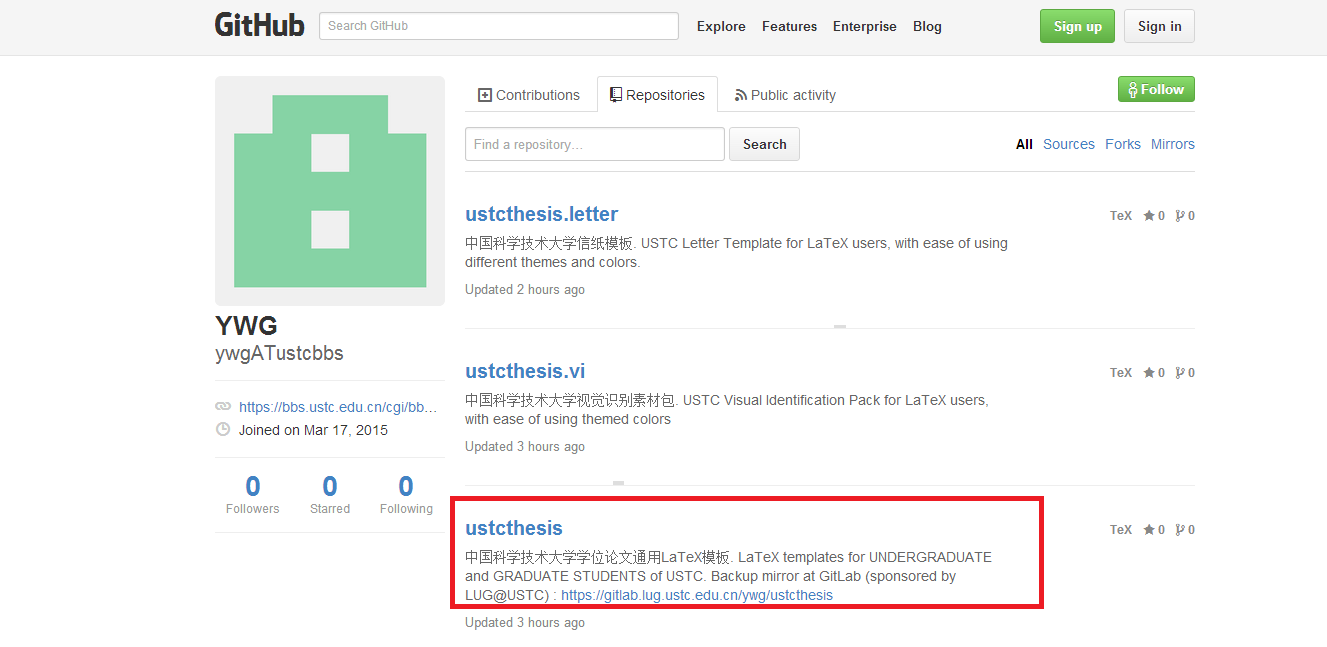
\includegraphics[width=\textwidth]{download}
\end{minipage}
\end{minipage}


\begin{tabular}{cc}
  \raisebox{-.1cm}{\begin{minipage}{.5\textwidth}
    \begin{Codex}[label=a.cpp, numbers=left]
      %#include "opencv2/highgui/highgui.hpp"
      %#include "opencv2/imgproc/imgproc.hpp"
      %#include <iostream>
      using namespace cv;
      using namespace std;
      int main(void)
      %{
          Mat img = imread("example.jpg", 0);
          imshow("example", img);
          waitKey();
          return 0;
    %  }
    \end{Codex}
  \end{minipage}} &
  \begin{minipage}{.5\textwidth}
    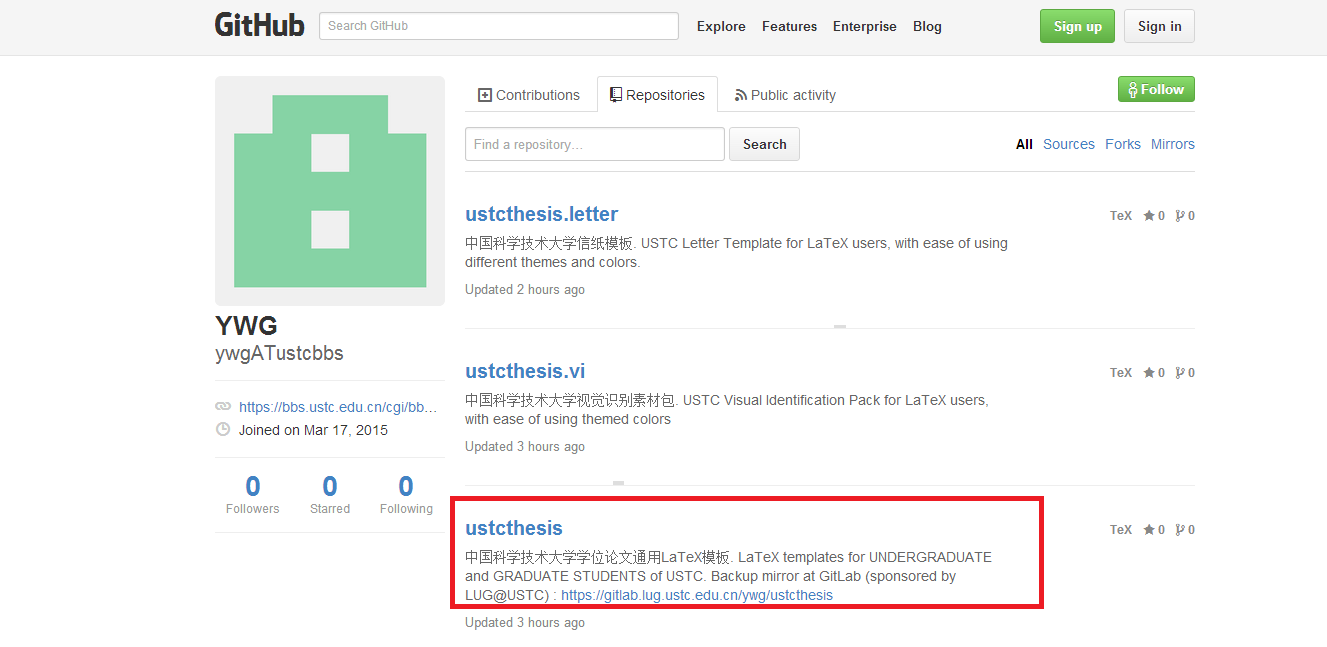
\includegraphics[width=\textwidth]{download}
  \end{minipage}
\end{tabular}
\fi



\section{数据加载模块}  %500字
可添加简单的容错处理

\section{版面分析模块}  % 3000字
\subsection{方案选取}


\section{预处理模块}     % 1000字
\subsection{方案选取}


\section{OCR模块}     % 6000字
\subsection{方案选取}

\section{字段解析模块}  %3000字
当含有文本的图片数据经过OCR模块以后,会被转换为文本,这些文本需要进行一定的加工,才能得到我们想要的各字段数据。总体来说,原始的文本需要经过数据清洗、字段匹配、目标文本提取等步骤。我们也可以认为这是数据的“后处理”过程。

\subsection{数据清洗}
数据清洗主要有两大功能,一是对文本的冗余信息(如因为图片噪声而产生的冗余符号)进行剔除,二是对文本进行简单的矫正。这两部分实现难度不大,却对之后的字段匹配过程有着很大的帮助。
\subsubsection{冗余信息剔除}
\subsubsection{文本矫正}

\subsection{字段匹配}
某段文本属于哪一个字段呢?这就需要对文本的具体内容进行理解划分了,例如若要判断
\subsubsection{StartsWith匹配}
\subsubsection{Includes匹配}


\section{数据存储模块} %500字
